\documentclass[12pt]{article}

\title{Anonymized title}
\author{Anonymous}
\date{\today}
\usepackage{listings}
\usepackage{xcolor}

\usepackage{graphicx}
\usepackage{setspace}
\usepackage{amsmath}
\usepackage{url}
\usepackage[margin=1in]{geometry}
\begin{document}


%\doublespace


\maketitle



\section{Escape paths that do not reach infinity}

As discussed in many papers, a 3D scalar field of quaternion magnitudes (e.g. $|Z|$) results from calculating a quaternion fractal set when using a finite 3D lattice of regularly spaced points as input.

Here we will visualize the escape paths for those points that maintain a quaternion magnitude less than the infinity threshold value (e.g. $4.0$) during the iteration process (e.g. $8$ iterations).

Here we will use Bezier curves and cylinders to draw the escape paths.
The length of these `shaggy' escape paths will be shortened to only $20\%$ of the total length, giving the impression of an isotropic buzz cut.

\pagebreak

\section{Core C++ code}

\lstset { %
    language=C++,
    backgroundcolor=\color{black!5}, % set backgroundcolor
    basicstyle=\footnotesize,% basic font setting
}

The C++ code to get a point along a Bezier curve, given by iforce2d on stackoverflow.com, is:
\begin{lstlisting}
vector_3 get_bezier_point(vector<vector_3> points, const float t)
{
	int i = points.size() - 1;

	while (i > 0)
	{
		for (int k = 0; k < i; k++)
		{
			points[k].x += t * (points[k + 1].x - points[k].x);
			points[k].y += t * (points[k + 1].y - points[k].y);
			points[k].z += t * (points[k + 1].z - points[k].z);
		}

		i--;
	}

	return points[0];
}
\end{lstlisting}

%\pagebreak

The C++ code for drawing a cylinder in OpenGL 1.x, given by jyk on gamedev.net, is:
\begin{lstlisting}
static const float rad_to_deg = 180.0f/pi;

vector_3 line = pos[i][j + 1] - pos[i][j];
			
glPushMatrix();

	glTranslatef(pos[i][j].x, pos[i][j].y, pos[i][j].z);

	const float line_len = line.length();
	line.normalize();
			
	float yaw = 0.0f;

	if (fabsf(line.x) < 0.00001 && fabsf(line.z) < 0.00001)
		yaw = 0.0f;
	else
		yaw = atan2f(line.x, line.z);

	float pitch = -atan2f(line.y, sqrtf(line.x*line.x + line.z*line.z));

	glRotatef(yaw*rad_to_deg, 0.0f, 1.0f, 0.0f);
	glRotatef(pitch*rad_to_deg, 1.0f, 0.0f, 0.0f);

	gluCylinder(glu_obj, 0.005, 0.005, line_len, 20, 2);

glPopMatrix();
\end{lstlisting}



\begin{figure} 
  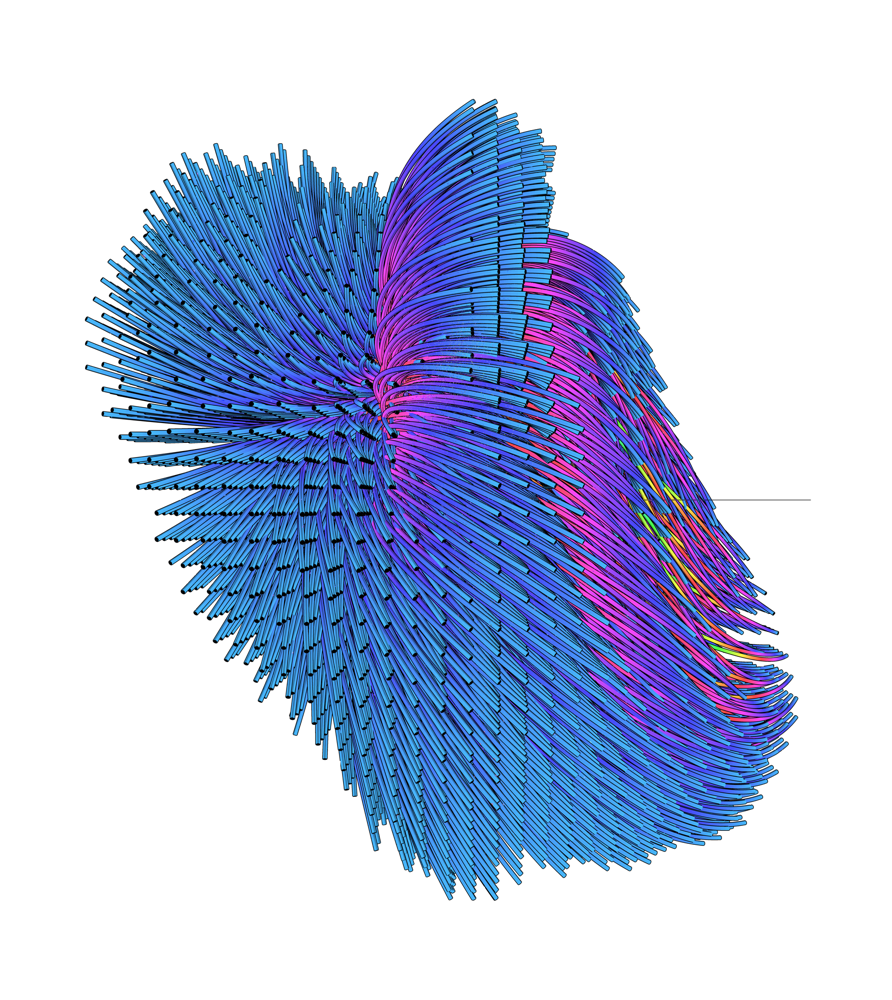
\includegraphics[width=\textwidth]{1.png}	
  \caption{$Z' = Z^2 + C$, where $C_{xyzw} = 0.3, 0.5, 0.4, 0.2$.}
\end{figure}

\begin{figure} 
  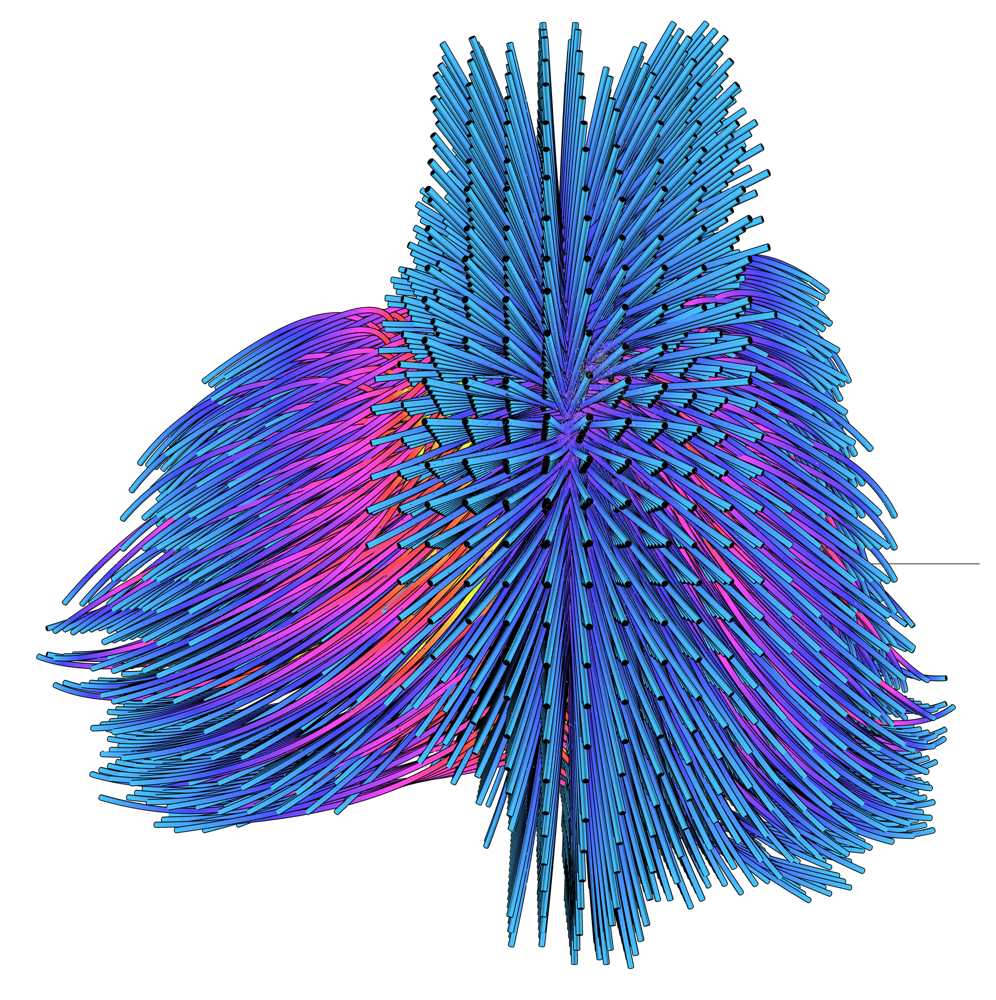
\includegraphics[width=\textwidth]{2.png}	
  \caption{$Z' = Z^3 + C$, where $C_{xyzw} = 0.3, 0.5, 0.4, 0.2$.}
\end{figure}

\begin{figure} 
  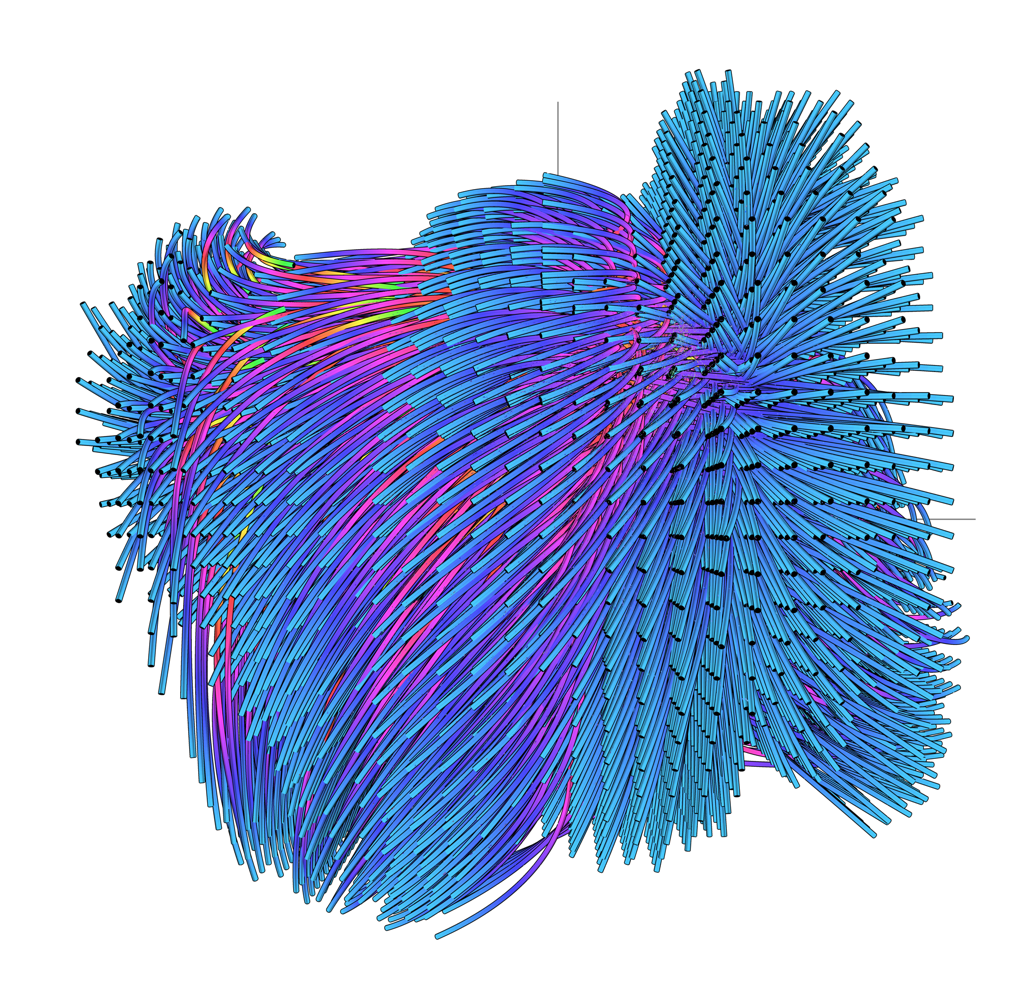
\includegraphics[width=\textwidth]{3.png}	
  \caption{`Pinhead': $Z^{\prime} = Z^4 + C$, where $C_{xyzw} = 0.3, 0.5, 0.4, 0.2$.}
\end{figure}

\begin{figure} 
  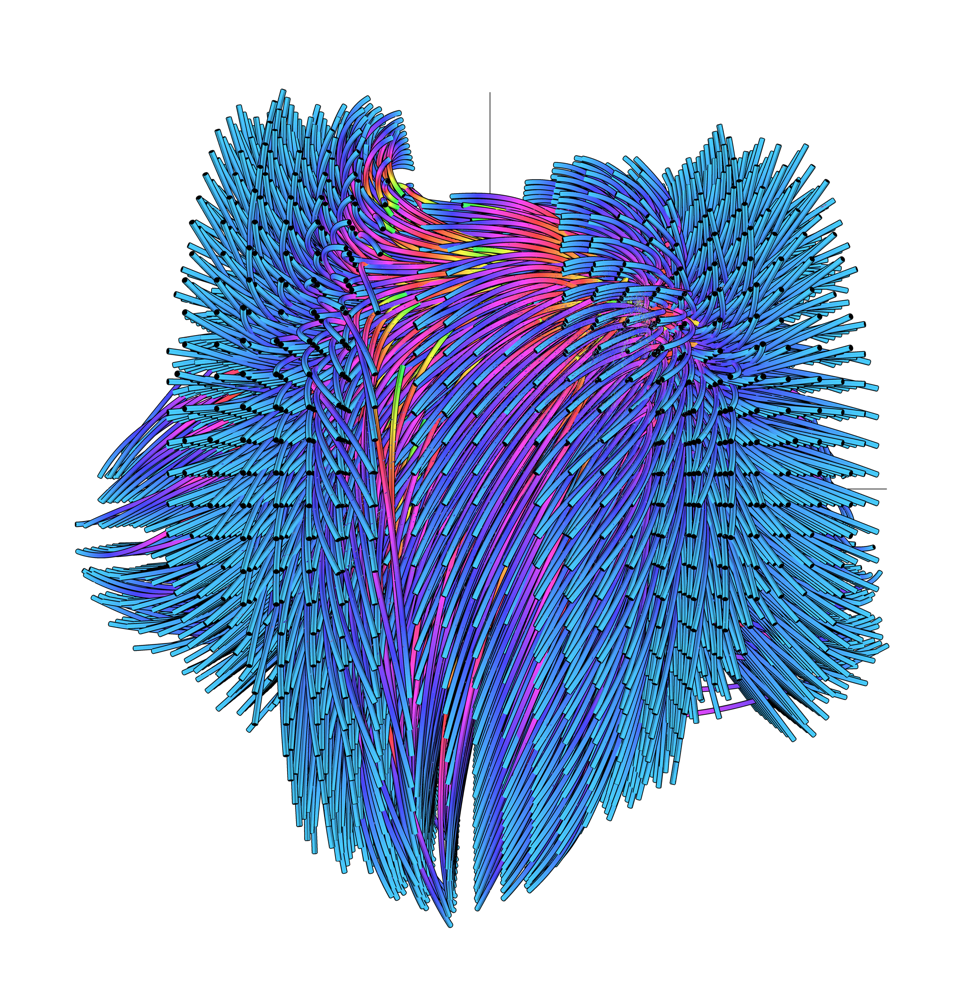
\includegraphics[width=\textwidth]{4.png}	
  \caption{$Z' = Z^5 + C$ , where $C_{xyzw} = 0.3, 0.5, 0.4, 0.2$.}
\end{figure}

\begin{figure} 
  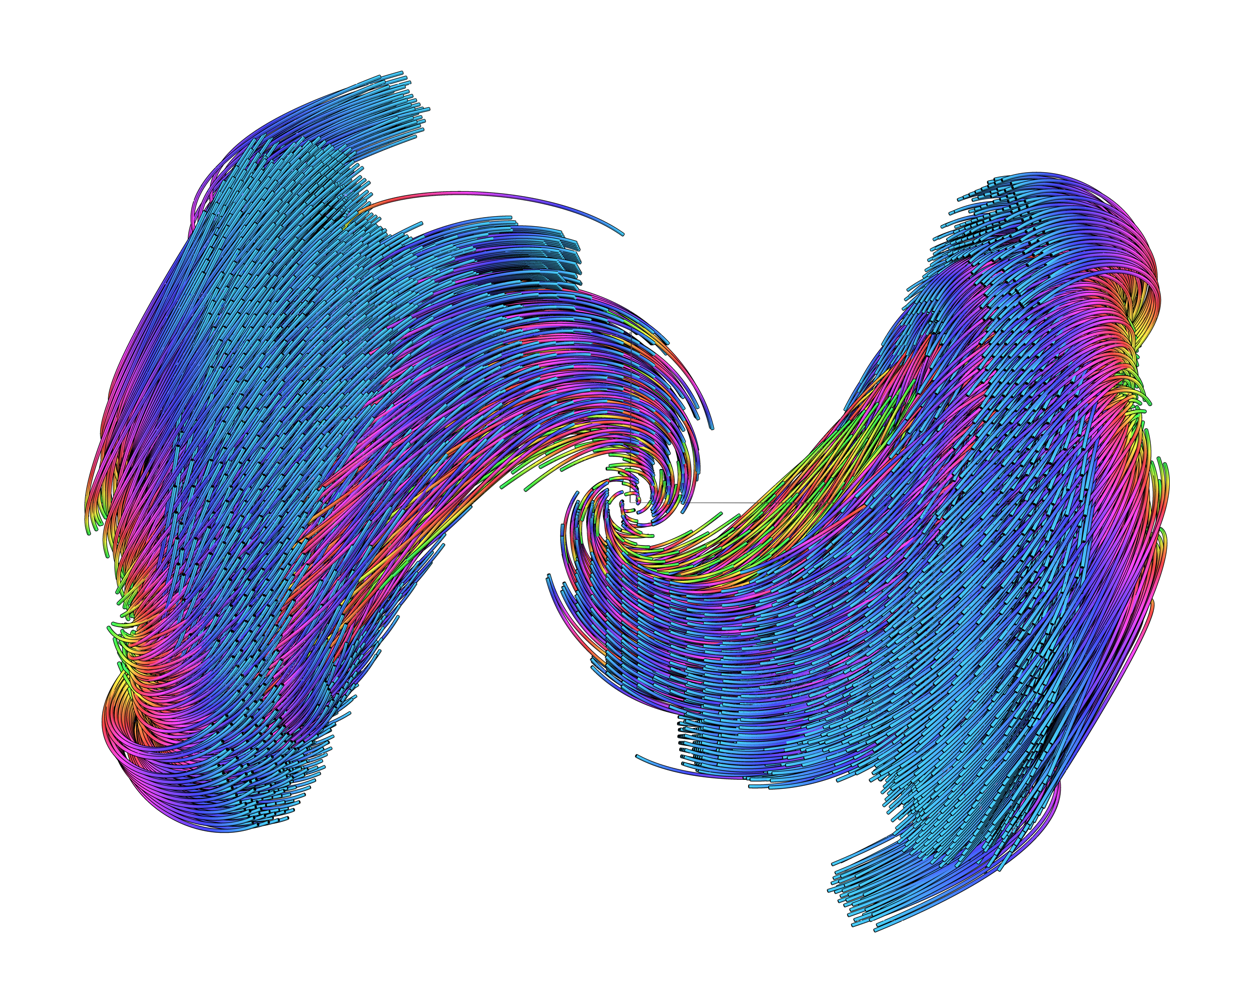
\includegraphics[width=\textwidth]{5.png}	
  \caption{$Z' = \sin(Z) + C\cdot\sin(Z)$, where $C_{xyzw} = 0.3, 0.5, 0.4, 0.2$.}
\end{figure}
 


%\begin{thebibliography}{9}
%\end{thebibliography}


\end{document}

